\documentclass[11pt]{article}
\usepackage[a4paper,margin=21mm]{geometry}
\usepackage[no-math]{fontspec}
\setmainfont{Latin Modern Roman}
\newfontfamily\CJKfont{Noto Serif CJK SC}
\XeTeXlinebreaklocale "zh"
\XeTeXlinebreakskip=0pt plus 1pt
\usepackage{amsmath,amssymb,amsthm,amscd,graphicx,color}
\usepackage{xurl}
\usepackage[unicode,hidelinks]{hyperref}
\allowdisplaybreaks
\setlength\emergencystretch{3em}
\numberwithin{equation}{section}

\usepackage{multirow}
\usepackage{mathtools}
\usepackage{tikz-cd}
\usepackage{stackrel}

\newtheorem{Theorem}{Theorem}[section]
\newtheorem*{Theorem*}{Theorem}
\newtheorem{Corollary}[Theorem]{Corollary}
\newtheorem{Lemma}[Theorem]{Lemma}
\newtheorem{Proposition}[Theorem]{Proposition}
 { \theoremstyle{definition}
\newtheorem{Definition}[Theorem]{Definition}
\newtheorem{Example}[Theorem]{Example}
\newtheorem{Remark}[Theorem]{Remark}
}

\newcommand{\SN}{\mathbb{N}} % Natural numbers
\newcommand{\SZ}{\mathbb{Z}} % Integers
\newcommand{\SQ}{\mathbb{Q}} % Rational numbers
\newcommand{\SR}{\mathbb{R}} % Real numbers
\newcommand{\SC}{\mathbb{C}} % Complex numbers
\newcommand{\C}{\SC} % Complex numbers
\newcommand{\SH}{\mathbb{H}} % Quaternions
\newcommand{\SO}{\mathbb{O}} % Octonions
\newcommand{\SP}{\mathbb{P}} %
\newcommand{\SA}{\mathbb{A}} %
\newcommand{\CZ}{\mathcal{Z}} %
\newcommand{\CC}{\mathcal{C}} %

\newcommand{\Rho}{\mathrm{P}}

\newcommand{\End}{\operatorname{End}}
\newcommand{\GL}{\operatorname{GL}}
\newcommand{\head}{\operatorname{h}}
\newcommand{\Hom}{\operatorname{Hom}}
\newcommand{\rank}{\operatorname{rank}}
\newcommand{\Rep}{\operatorname{Rep}}
\newcommand{\SL}{\operatorname{SL}}
\newcommand{\Sym}{\operatorname{Sym}}
\newcommand{\tail}{\operatorname{t}}
\newcommand{\im}{\operatorname{im}}
\newcommand{\jer}{\operatorname{ker}}

\newcommand{\PiGamma}{B}
\newcommand{\PiQ}{A}

\DeclareMathOperator{\module}{\mathrm{-mod}}
\DeclareMathOperator{\Hilb}{\mathrm{Hilb}}
\DeclareMathOperator{\Quot}{\mathrm{Quot}}

\newcommand{\QuotI}[1][ ]{\Quot_I^{#1}}
\newcommand{\QuotInI}{\QuotI[n_I]}
\newcommand{\Quoti}[1][ ]{\Quot_i^{#1}}
\newcommand{\Quotini}{\Quoti[n_i]}
\newcommand{\vprime}{v'}

\numberwithin{equation}{section}

\mathchardef\mhyphen="2D
\newcommand{\ngammahilb}{n\Gamma\mhyphen\Hilb\big(\SC^2\big)}


\makeatletter\newlabel{prop:Qnrep}{{3.1}{}{Original source locator}{}{}}\makeatother
\begin{document}
\begin{center}\Large Reduced fine moduli of nonempty cornered framed McKay algebras are quiver varieties after the specified dimension-vector enlargement\end{center}
\noindent\textbf{Stable ID:} 1434\quad\textbf{Author:} Alastair Craw; Soren Gammelgaard; Adam Gyenge; Balazs Szendroi\par
\noindent\textbf{Work:} Quot Schemes for Kleinian Orbifolds\par
\noindent\textbf{Source:} \url{https://sigma-journal.com/2021/099/}\par
\noindent\textbf{Version:} Official SIGMA 17 (2021) article 099, DOI 10.3842/SIGMA.2021.099; journal PDF and native TeX acquired 2026-09-30, exact bytes pinned by SHA256\par
\noindent\textbf{Rights:} CC BY 4.0. Authors retain copyright. \url{https://creativecommons.org/licenses/by/4.0/}. Reuse and typesetting adaptation; original language and mathematical content preserved.\par
\noindent\textbf{Difficulty (prior selection preserved):} {\CJKfont H3: The proof constructs a suitable enlargement of a dimension vector by explicit inequalities on the affine McKay graph, then controls extensions across removed vertices using finite-type Cartan positivity. It combines dense-stratum resolution, recollement and polystable decompositions to prove surjectivity of a previously constructed closed immersion. The reduced-scheme qualification and enlargement are essential; ordinary cornering or variation of GIT alone does not prove the result.}\par
\medskip\noindent\textbf{Editorial boundary note (not author text):} Selected author-main Theorem6.9 reduced-scheme identification of nonempty cornered framed McKay fine moduli with the quiver variety after the specified dominating dimension-vector enlargement. Full complex-field/stability/dimension-vector/McKay/preprojective/cornered algebra/fine-moduli conventions, original Hilbert-component definition, GIT/wall parameters, complete dense-stratum resolution and line-bundle factorization, closed immersion, dominating vector construction in all three cases, recollement/polystable extension, Cartan bound and final closed-point surjectivity are retained. Existing Nakajima/GIT/finite-type Cartan facts and precise prior Craw et al.2021 lemmas/proposition are preserved as references with the current authors explicit dimension-vector-independent application; no editor construction is inserted. Supporting resolution/inequalities/functors have no extra counts, and orbifold Quot equivalence/downstream variants are unselected. Original final K-complement versus union wording discrepancy remains literal alongside the preceding exact complement definition; no formula repair. All required diagrams remain author-coded editable TikZ. Only an unused preamble remarks declaration with a nonexistent lowercase theorem counter is omitted; no active author environment or mathematics is changed.\par
\noindent\textbf{External original reference prop:Qnrep:} Original unselected basic associative-Quot representability Proposition3.1/native321–363, mentioned only in the author introduction as another contribution. It is not a premise of selected Theorem6.9.\par
\medskip\hrule\medskip\noindent\textbf{Author text begins below.}\par
\setcounter{section}{1}
% Original source lines 132--140
In this paper, we have three main goals.
First, we aim to
understand better the moduli spaces $\mathcal{M}_{\PiQ_I}$,
constructing them as a kind of Quot scheme
that is both natural and geometric.
Second, with applications in mind, we consider arbitrary dimension vectors, not just multiples of some set of fixed dimension vectors as above. One interpretation of our results is a new fine moduli space structure, as well as a (noncommutative)
geometric interpretation, of a large class of
Nakajima quiver varieties for certain non-generic stability parameters.
Our third and final goal is to provide proofs that completely bypass any case-by-case analysis of ADE diagrams.


% Original source lines 177--188
While some of our
arguments follow~\cite{craw2019punctual} closely,
we introduce
Quot schemes in a general noncommutative
context, establishing a basic representability result in Proposition~\ref{prop:Qnrep} that may be of broader interest. Furthermore, while the
morphism
\[ \mathfrak{M}_\theta(1,v) \longrightarrow \mathfrak{M}_{\theta_I}(1,v) \]
induced by varying a generic stability condition $\theta$ to a special one $\theta_I$ is always surjective for the
dimension vector $v=n\delta$ relevant to the case $\Hilb^n\big(\SC^2/\Gamma\big)$ discussed above,
the same is not true in general.
Instead, one has to correct $v$ to
obtain a surjective morphism of quiver varieties.


% Original source lines 213--272
\noindent
\textbf{Conventions.}
 We work throughout over $\SC$. In particular, all schemes are $\SC$-schemes and all tensor products are taken over $\SC$ unless otherwise indicated. We often use the following partial order on dimension vectors: for any $n\in \mathbb{N}$ and for $u=(u_i),v=(v_i)\in \mathbb{Z}^n$, we define $u\le v$ if $u_i\le v_i$ for all $1\leq i\leq n$. We adopt the sign convention of King~\cite{king1994moduli} for $\theta$-stability, so a~module $M$ over an algebra is $\theta$-stable (resp.\ $\theta$-semistable) if $\theta(M)=0$ and every nonzero proper submodule $N\subsetneq M$ satisfies $\theta(N)>0$ (resp.\ $\theta(N)\ge 0$).

\section{Preliminaries}\label{sec:prelim}

\subsection{Three algebras arising from the McKay graph}\label{subsec:mckay}
Let $\Gamma\subset \GL(V)$ be a finite subgroup of the general linear group for an $m$-dimensional $\SC$-vector space $V$.
Choosing a basis of $V$, we can write the symmetric algebra of the dual vector space $V^*$ as a polynomial ring $R=\SC[x_1,\dots,x_m]$. The group $\Gamma$ acts dually on $R$: for $g\in \Gamma$ and $f\in R$, we have $(g\cdot f)(v) = f\big(g^{-1} v\big)$ for all $v\in V$. Let $R^\Gamma$ denote the $\Gamma$-invariant subring of~$R$.

List the irreducible representations of $\Gamma$ as $\{\rho_0, \rho_1, \dots, \rho_r\}$, where $\rho_0$ is the trivial representation.
The decomposition of $R$ as an $R^\Gamma$-module can be written \cite[Proposition~4.1.15]{goodman2009symmetry}
 \begin{gather*} %\label{eqn:decompR}
 R\cong \bigoplus_{0\leq i\leq r} R_i\otimes_\mathbb{C} \rho_i,
 \end{gather*}
 where $R_i\coloneqq \Hom_\Gamma(\rho_i,R)$ is an
 $R^\Gamma$-module; note that $R_0=R^{\Gamma}$.

From now on, let $\Gamma \subset \SL(2,\SC)$ be a finite subgroup acting as above on $R=\SC[x,y]$. The \emph{McKay graph} of $\Gamma$
has vertex set $\{0,1, \dots, r\}$ corresponding to the irreducible representations of~$\Gamma$, where for each $0\leq i, j\leq r$, we have $\dim\Hom_{\Gamma}(\rho_j , \rho_i \otimes V )$ edges joining vertices~$i$ and~$j$. McKay~\cite{McKay80} observed that this graph is an affine Dynkin diagram of ADE type. We frame this graph by introducing an additional vertex, denoted~$\infty$, together with an edge joining the vertices~$\infty$ and~$0$; we refer to the resulting graph as the \emph{framed McKay graph} of~$\Gamma$.

We now associate a doubled quiver to each graph. For this, consider
the set of pairs $Q_1$ comprising an edge in the framed McKay graph
and an orientation of the edge. For each $a\in Q_1$, we write~$t(a)$,
$h(a)$ for the vertices at the tail and head respectively of
the oriented edge, and we write $a^{\ast}$ for the same edge with
the opposite orientation. Define the \emph{framed McKay quiver of $\Gamma$},
denoted $Q$, to be the quiver with vertex set $Q_0= \{\infty,0,\dots ,r\}$
and arrow set $Q_1$. The (unframed) \emph{McKay quiver},
denoted $Q_\Gamma$, is the complete subquiver of $Q$ on
the vertex set $\{0, 1,\dots, r\}$. Using these quivers
we define the following three algebras.

First, let $\SC Q$ denote the path algebra of the framed McKay quiver $Q$. For $i \in Q_0$, let $e_i \in \SC Q$ denote the idempotent corresponding to the trivial path at vertex $i$. Let $\epsilon\colon Q_1 \to \{\pm 1\}$ be any map such that $\epsilon(a) \neq \epsilon(a^{\ast})$ for all $a \in Q_1$. The \emph{preprojective algebra of $Q$}, denoted $\Pi$, is defined as the quotient of $\SC Q$ by the ideal
\begin{equation}
\label{eqn:preprojectiverelation}
\left\langle \sum_{\head(a)=i} \epsilon(a) aa^{\ast} \mid {i \in Q_0}
\right\rangle.
\end{equation}
 The preprojective algebra $\Pi$ does not depend on the choice of the map $\epsilon$. For each $i\in Q_0$, we simply write $e_i\in \Pi$ for the image of the corresponding vertex idempotent.

Second, in the framed McKay quiver $Q$, let $b^*\in Q_1$ be the unique arrow with head at vertex~$\infty$. Define a $\SC$-algebra as the quotient of the preprojective algebra $\Pi$ by the two-sided ideal generated by the class of $b^*$:
 \[
 \PiQ\coloneqq \Pi/(b^*).
 \]
 Equivalently, if we define a quiver $Q^*$ to have vertex set $Q^*_0=\{\infty,0,1,\dots,r\}$ and arrow set $Q_1^*=Q_1\setminus \{b^*\}$, then $\PiQ$ is the quotient of the path algebra $\SC Q^*$ by the ideal of relations
 \begin{equation*}% \label{eqn:Arelations}
 \left\langle \sum_{\head(a) = i} \epsilon(a) aa^* \mid 0\leq i,
 \head(a^*)\leq r \right\rangle.
 \end{equation*}

 Third, let $\SC Q_\Gamma$ denote the path algebra of the (unframed) McKay quiver $Q_\Gamma$. Since $\SC Q_\Gamma$ is a subalgebra of $\SC Q$, we use the same symbol $e_i\in \SC Q_\Gamma$ for the idempotent corresponding to the trivial path at vertex $i$ of $Q_\Gamma$. The \emph{preprojective algebra of $Q_\Gamma$}, denoted $\PiGamma$, is defined as the quotient of $\SC Q_\Gamma$ by an ideal defined similarly to that from~\eqref{eqn:preprojectiverelation} for the quiver $Q_\Gamma$.

\begin{Remark}
 For each vertex $0\leq i\leq r$ we denote by $e_i$ the class in $\PiQ$ of the idempotent at the vertex $i$. Note that $\PiGamma$ is not a subalgebra of $\Pi$. On the other hand, $\PiGamma$ is isomorphic to the subalgebra $\oplus_{0 \leq i,j \leq r} e_j\PiQ e_i$ of $\PiQ$ due to \cite[Lemma~3.2]{craw2019punctual}, and moreover
 \begin{equation} \label{eq:PiQdecomp}
 \PiQ \cong \PiGamma \oplus \PiGamma b \oplus \SC e_\infty.
\end{equation}
as complex vector spaces. In particular, the classes $e_i$, $0 \leq i \leq r$ are also contained in $\PiGamma$.
\end{Remark}

\setcounter{section}{3}\setcounter{subsection}{2}
% Original source lines 426--429
 Denote by $\Hilb\big(\big[\SC^2/\Gamma\big]\big)$ the Hilbert scheme of $\Gamma$-invariant finite colength subschemes of~$\SC^2$. As explained in more detail in \cite[Section~1.1]{gyenge2018euler}, this space decomposes as a disjoint union of quasi-projective varieties
\[\Hilb\big(\big[\SC^2/\Gamma\big]\big) = \coprod_{v\in \mathbb{N}^{r+1}}\Hilb^v\big(\big[\SC^2/\Gamma\big]\big),
\]
where \[\Hilb^v\big([\SC^2/\Gamma]\big) =\Big\{J\in \Hilb\big(\big[\SC^2/\Gamma\big]\big)\mid H^0\big(\mathcal{O}_{\SC^2}/J\big) \cong \bigoplus_{i\in \{0, \dots, r\}} \rho_i^{\oplus v_i}\Big\}.\]


% Original source lines 490--530
\section{Fine moduli spaces of modules}
\label{subsec:finemod}

\subsection{Cornering and fine moduli spaces}

Let $\Rep(\Gamma)$
denote the representation ring of $\Gamma$. Introduce a formal symbol $\rho_{\infty}$ so that $\{\rho_i \mid i \in Q_0\}$ provides a $\mathbb{Z}$-basis for $\mathbb{Z}^{Q_0}\cong \mathbb{Z}\oplus \Rep(\Gamma)$ considered as $\mathbb{Z}$-modules.

Recall that $\PiQ=\Pi/(b^{\ast})$ is the quotient of the
preprojective algebra of the framed McKay quiver of $\Gamma$ by the two sided ideal $(b^{\ast})$, where $b^\ast$ is the arrow from $0$ to $\infty$.
Let $I \subseteq \{0, \dots , r\}$ be a non-empty subset; we work under the assumption that $I\ne \varnothing$ for the rest of the paper.
Define the idempotent $\overline{e}_I \coloneqq e_{\infty} + \sum_{i \in I} e_i \in \PiQ$.
The subalgebra
\begin{equation}\label{eqn:AI}
\PiQ_I \coloneqq \overline{e}_I \PiQ \overline{e}_I
\end{equation}
of $A$ comprises linear combinations of
classes of paths in $Q$ whose tails and heads lie in the set $\{\infty\} \cup I$; this is also an instance of \emph{cornering}~\cite[Remark~3.1]{craw2018multigraded}.

Let
$n_I \coloneqq {(n_i)_{i\in I}}= \sum_{i \in I} n_i \rho_i \in \mathbb{N}^{I}$.
Then $(1,n_I)\coloneqq\rho_{\infty} +n_I \in \mathbb{N} \oplus \mathbb{N}^{I}$
is a dimension vector for $\PiQ_I$-modules, and we consider the stability condition $\eta_{I}\colon \mathbb{Z} \oplus \mathbb{Z}^{I} \to \mathbb{Q}$
given by
\begin{equation}
 \label{eqn:etaI}
\eta_I (\rho_i) =
\begin{cases}
\displaystyle -\sum_{j \in I} n_j & \textrm{for } i= \infty, \\
1 & \textrm{if }i \in I.
\end{cases}
\end{equation}

It follows directly from the definition that an $\PiQ_I$-module $N$ of dimension vector $(1,n_I)$ is $\eta_I$-stable if and only if
there exists a surjective $\PiQ_I$-module homomorphism $\PiQ_I e_{\infty} \to N$.
The quiver moduli space construction of King~\cite[Proposition~5.3]{king1994moduli} for finite dimensional algebras can be adapted to any algebra presented as the quotient of a finite, connected quiver by an ideal of relations. We established in \cite[Proposition~3.3]{craw2019punctual} that the algebra $\PiQ_I$ has this property.
The vector~$(1,n_I)$ is indivisible and $\eta_I$ is a generic stability condition for $\PiQ_I$-modules of dimension vector~$(1,n_I)$, so there is a~fine moduli space $\mathcal{M}_{\PiQ_I}(1,n_I)$
of $\eta_I$-stable $\PiQ_I$-modules of dimension
vector~$(1,n_I)$. Let $T_I \coloneqq\bigoplus_{i \in \{\infty \}\cup I } T_i$ denote the tautological vector bundle on~$\mathcal{M}_{\PiQ_I}(1,n_I)$, where~$T_{\infty}$ is the trivial bundle and $T_i$ has rank~$n_i$ for $i \in I$.
After multiplying $\eta_I$ by a positive integer $m\geq 1$ if necessary, we may assume that the polarising ample line bundle $\mathcal{L}_I \coloneqq \bigotimes_{i \in I} \mathrm{det}(T_i)^{m}$ on $\mathcal{M}_{\PiQ_I}(1,n_I)$ given by the GIT construction is very ample.



% Original source lines 605--1011
\section{Quiver varieties for the framed McKay quiver}\label{sec:quivers}

\subsection{Variation of GIT quotient for quiver varieties}
\label{subsec:quivervars}

Let $v\coloneqq(v_i)_{0 \leq i \leq r} \in \mathbb{N}^{r+1}$ be a dimension vector for the McKay quiver $Q_\Gamma$.
Recall that we identify $\mathbb{Z}^{Q_0}\cong \mathbb{Z}\rho_{\infty}\oplus \Rep(\Gamma)$, so we obtain the
dimension vector \[(1,v) \coloneqq\rho_{\infty}+\sum_{i=0}^r v_i\rho_i \in \mathbb{N}^{Q_0}
\] for the framed McKay quiver $Q$. Write
\[ \Theta_{v}=\big\{\theta\colon \mathbb{Z}^{Q_0} \to \mathbb{Q}\; : \; \theta\big((1,v)\big)=0 \big\} \]
for the space of stability conditions for the
the framed quiver. Following Nakajima~\cite{nakajima1994instantons, Nakajima98}, for every $\theta \in \Theta_{v}$, the quiver variety $\mathfrak{M}_{\theta}(1,v)$ is the coarse moduli space of S-equivalence classes of $\theta$-semistable $\Pi$-modules of dimension vector $(1,v)$. The GIT construction of $\mathfrak{M}_{\theta}(1,v)$ is summarised for example in \cite[Section 2]{craw2019punctual}; see also \cite[Section 2]{nakajima2009quiver}. Note in particular that we give $\mathfrak{M}_{\theta}(1,v)$ the reduced scheme structure.


The set of stability conditions $\Theta_v$ admits a preorder $\geq$, and this determines a wall-and-chamber structure, where
$\theta,\theta' \in \Theta_v$ lie in the relative interior of the same cone if and only if both $\theta \geq \theta'$ and $\theta' \geq\theta$ hold in this preorder, in which case $\mathfrak{M}_{\theta}(1,v)\cong\mathfrak{M}_{\theta'}(1,v)$. The interiors of the top-dimensional cones in $\Theta_v$ are chambers, while the codimension-one faces of the closure of each chamber are walls. We say that $\theta \in \Theta_v$ is generic with respect to $v$, if it lies in some GIT chamber. The vector $(1,v)$ is indivisible, so again, \cite[Proposition~5.3]{king1994moduli} implies that for generic $\theta \in \Theta_v$ the quiver variety $\mathfrak{M}_{\theta}(1,v)$ is the fine moduli space of isomorphism classes of $\theta$-stable $\Pi$-modules of dimension vector $(1,v)$. In this case, the universal family on $\mathfrak{M}_{\theta}(1,v)$ is a tautological locally-free sheaf $\mathcal{R} \coloneqq \oplus_{i \in Q_0}\mathcal{R}_i$ together with a $\SC$-algebra homomorphism $\varphi \colon \Pi \to \mathrm{End}(\mathcal{R})$, where $R_\infty$ is the trivial bundle on $\mathfrak{M}_{\theta}(1,v)$ and where $\mathrm{rank}(\mathcal{R}_i) = v_j$ for $i \geq 0$.

\begin{Lemma}\label{lem:quiver}\quad
\begin{enumerate}\itemsep=0pt
\item[$1.$] For all $\theta \in \Theta_v$, the scheme $\mathfrak{M}_{\theta}(1,v)$ is irreducible and normal, with symplectic singularities.
\item[$2.$] Let $ \theta \geq \theta'$. The morphism $\pi\colon \mathfrak{M}_{\theta}(1,v) \to \mathfrak{M}_{\theta'}(1,v)$ obtained by variation of GIT quotient is a projective morphism of varieties over the affine quotient $\mathfrak{M}_{0}(1,v)$.
\end{enumerate}
\end{Lemma}

\begin{proof}
Part (1) is \cite[Theorem 1.2, Proposition 3.21]{bellamy2016symplectic} while part (2) is well-known.
\end{proof}

\subsection{Wall-and-chamber structure}
\label{subsec:wallandcham}

Define $\delta\coloneqq \sum_{0\leq i\leq r} \dim(\rho_i)\rho_i\in \Rep(\Gamma)$. For the dimension vector $v\coloneqq n\delta$, the GIT wall-and-chamber structure on $\Theta_{n\delta}$ is computed explicitly in \cite[Theorem 4.6]{bellamy2020birational}. More generally, for arbitrary $v \in \mathbb{N}^{r+1}$,
it is possible to compute the wall-and-chamber structure on $\Theta_v$ by applying recent work of
Dehority~\cite[Proposition 4.8]{dehority2020affinizations}. We do not need the wall-and-chamber structure here, but we do use the following distinguished region of the space of stability conditions:
\[ C^{+}_v\coloneqq \{\theta \in \Theta_v \mid \theta(\rho_i) > 0 \textrm{ for } 0 \leq i \leq r \}. \]
This open cone need not be a GIT chamber, though it is always contained in one (and it is a chamber in the special case $v=n\delta$, see \cite[Example~2.1]{bellamy2020birational} or \cite[Section~2.8]{nakajima2009quiver}).
The next statement, which appeared originally in \cite[Section~2]{nakajima2002geometric}, illustrates the importance of $C^{+}_v$.
\begin{Proposition}
\label{prop:hilbiso}
For $v \in \mathbb{N}^{r+1}$ and $\theta \in C^{+}_v$, there is an isomorphism
\[ \Hilb^{v}\big(\big[\SC^2/\Gamma\big]\big) \cong \mathfrak{M}_{\theta}(1,v). \]
\end{Proposition}
\begin{proof}
In the special case $v=n\delta$,
the statement is proved in \cite[Theorem 4.6]{kuznetsov2007quiver}. However, the argument given there applies for
an arbitrary dimension vector $v$; note in particular that the auxiliary \cite[Corollary 3.5]{kuznetsov2007quiver}
does not need any assumption on the dimension vector (and we have that $\Hilb^{v}\big(\big[\SC^2/\Gamma\big]\big)$ is non-empty if and only if $\mathfrak{M}_{\theta}(1,v)$ is non-empty).
\end{proof}

Every face of the closed cone $\overline{C^{+}_v}$ is of the form
\[ \sigma_I\coloneqq\big\{\theta \in \overline{C^{+}_v} \mid \theta(\rho_i) > 0 \textrm{ if and only if } i \in I, \textrm{ and } \theta(\rho_i) = 0 \textrm{ otherwise} \big\} \]
for some non-empty subset $I \subseteq\{0,\dots,r\}$. When $v=n\delta$, these faces are contained in walls of the wall-and-chamber structure on $\Theta_{n\delta}$, though this need not be the case for arbitrary $v \in \mathbb{N}^{r+1}$.
In any case, the parameter
\begin{equation} \label{eqn:theta_I}
\theta_I (\rho_j) \coloneqq
\begin{cases}
\displaystyle -\sum_{i \in I} v_i & \textrm{for }j=\infty, \\
1 & \textrm{if } j \in I, \\
0 & \textrm{if } j \in \{0,1,\dots,r\} \setminus I
\end{cases}
\end{equation}
lies in the relative interior of the face $\sigma_I$.

\subsection{Resolution of singularities}
Let $v \in \mathbb{N}^{r+1}$ be a dimension vector and $I \subseteq \{0, \dots , r\}$. As mentioned above, the quiver variety $\mathfrak{M}_{\theta_I}(1,v)$ is singular in general for $\theta_I$ as defined in \eqref{eqn:theta_I} above. Moreover, for $\theta\in C_v^+$,
the morphism
\[ \mathfrak{M}_{\theta}(1,v) \to \mathfrak{M}_{\theta_I}(1,v)\]
obtained by variation of GIT need not be birational.
It is nevertheless possible to find a resolution of $\mathfrak{M}_{\theta_I}(1,v)$ using a
quiver variety if one modifies the dimension vector~$v$:

\begin{Proposition}\label{prop:surjvar}
Let $v \in \mathbb{N}^{r+1}$ and let $ I \subseteq \{0, \dots , r\}$ be non-empty. Assume further that
$\mathfrak{M}_{\theta_I}(1,v)$ is non-empty.
There exists a dimension vector $\widetilde{v}\in \mathbb{N}^{r+1}$ satisfying $\widetilde{v}_i \leq v_i$ for $0 \leq i \leq r$ and $\widetilde{v}_i = v_i$ for $i \in I$,
such that there is a projective resolution of singularities
\[
\pi_{I}\colon \ \mathfrak{M}_{\widetilde{\theta}}(1,\widetilde{v})\to \mathfrak{M}_{\theta_I}(1,v),
\]
where the stability condition $\widetilde{\theta}$ satisfies $\widetilde\theta\in C_{\widetilde v}^+$.
\end{Proposition}
\begin{proof}
 Following Nakajima~\cite[Section 6]{nakajima1994instantons} (cf.\ \cite[Section 3.5]{bellamy2020birational}),
 there is a finite stratification
\begin{equation*}
\mathfrak{M}_{\theta_I}(1,v) = \coprod_{\gamma} \mathfrak{M}_{\theta_I}(1,v)_{\gamma} \end{equation*}
by smooth locally-closed subvarieties, where the union is over conjugacy classes of subgroups of the reductive group applied during the GIT construction of $\mathfrak{M}_{\theta_I}(1,v)$, and where the stratum $\mathfrak{M}_{\theta_I}(1,v)_{\gamma}$ consists of $S$-equivalence classes of semistable modules with polystable representative having stabiliser in the conjugacy class $\gamma$. Since $\mathfrak{M}_{\theta_I}(1,v)$ is irreducible by Lemma~\ref{lem:quiver}, there is a unique dense stratum and we fix a conjugacy class $\gamma$
 such that the dense open stratum in~$\mathfrak{M}_{\theta_I}(1,v)$ is $\mathfrak{M}_{\theta_I}(1,v)_\gamma$. Apply \cite[Proposition 2.25]{nakajima2009quiver} to obtain a dimension vector $\widetilde{v}\in \mathbb{N}^{r+1}$ as in the statement of the lemma
 together with an isomorphism
\begin{equation} \label{eqn:gammaIsom}
\mathfrak{M}_{\theta_I}(1,v)_{\gamma} \cong \mathfrak{M}^s_{\theta_I}(1,\widetilde{v}) \times {Y},
\end{equation}
 where $\mathfrak{M}^s_{\theta_I}(1,\widetilde{v})$ is the fine moduli space of $\theta_I$-stable $\Pi$-modules of dimension vector $(1,\widetilde{v})$, and ${Y} \subset \mathfrak{M}_{0}(0,v-\widetilde{v})$ is a locally-closed subvariety.
 Note that $\mathfrak{M}_{\theta_I}(1,v)_{\gamma}$ is non-empty by assumption, hence so are $\mathfrak{M}^s_{\theta_I}(1,\widetilde{v})$ and ${Y}$.

 We claim that ${Y}$ is a closed point. Indeed, $\mathfrak{M}_0(0, v-\widetilde{v})$ parametrises
 0-polystable representations, i.e., direct sums of simple representations. The framing is 0-dimensional,
and since~$I$ is non-empty, there is at least one $i$ such that $v_i = \widetilde{v}_i$. It follows that the representations parameterised by ${Y}$
are supported on a doubled quiver obtained from an affine ADE diagram with at least one vertex removed. Removing a vertex from an affine ADE diagram leaves a graph in which every connected component is a subgraph of an finite type ADE diagram. Therefore $\mathfrak{M}_0(0, v-\widetilde{v})$ parametrises direct sums of simple representations of preprojective algebras of doubled quivers associated to finite type ADE diagrams. A simple representation of any such quiver is one-dimensional \cite[Lemma~2.2]{savage2011quiver}, so the only polystable representation of dimension vector $(0, v-\widetilde{v})$ is
necessarily of the form
\begin{equation}\label{eqn:directsumsimples}
\bigoplus_{0\leq i\leq r}S_i^{\oplus(v_i-\tilde{v}_i)},
\end{equation}
where each $S_i$ is a vertex simple $\Pi$-module. Therefore $\mathfrak{M}_0(0, v-\widetilde{v})$ is a closed point, and hence so too is ${Y}$ because ${Y}\neq \varnothing$. Thus $\mathfrak{M}_{\theta_I}(1,v)_{\gamma} \cong \mathfrak{M}^s_{\theta_I}(1,\widetilde{v})$.

For
 $\widetilde\theta\in C_{\widetilde v}^+$, we claim that the desired morphism $\pi_I\colon \mathfrak{M}_{\widetilde{\theta}}(1,\widetilde{v})\to \mathfrak{M}_{\theta_I}(1,v)$ is induced by sending each $\tilde{\theta}$-stable $\Pi$-module $V$ of dimension vector $(1,\tilde{v})$ to
 \[
 \pi_I(V):=V\oplus\bigoplus_{0\leq i\leq r}S_i^{\oplus(v_i-\tilde{v}_i)}.
 \]
 Indeed, if $\tilde{\mu}$ and $\mu$ denote the moment maps for the actions of $G_{\tilde{v}}:=\prod_{0\leq i\leq r}\GL(\tilde{v}_i)$ and $G_{v}:=\prod_{0\leq i\leq r}\GL(v_i)$ on the representation spaces of $\Pi$-modules of dimension vectors $(1,\tilde{v})$ and $(1,v)$ respectively, then the above assignment induces an inclusion $\tilde{\mu}^{-1}(0)\hookrightarrow \mu^{-1}(0)$ that is equivariant with respect to the actions of $G_{\tilde{v}}$ and $G_v$ on $\tilde{\mu}^{-1}(0)$ and $\mu^{-1}(0)$ respectively. Any submodule of~$\pi_I(V)$ is $W\oplus W'$ for submodules $W\subseteq V$ and $W'\subseteq \bigoplus_{0\leq i\leq r}S_i^{\oplus(v_i-\tilde{v}_i)}$, and we have $\theta_I(W\oplus W') = \theta_I(W)\geq 0$. Thus, the image of the $\tilde{\theta}$-stable locus of $\tilde{\mu}^{-1}(0)$ lies in the $\theta_I$-semistable locus of~$\mu^{-1}(0)$, and this inclusion induces the morphism $\pi_I$ as claimed.

 It remains to establish the properties of $\pi_I$. Adapting the proof from \cite[Lemma~2.4]{bellamy2016symplectic} shows that~$\pi_I$ is a projective morphism, while \cite[Theorem~1.15]{bellamy2016symplectic} gives that $ \mathfrak{M}_{\widetilde{\theta}}(1,\widetilde{v})$ is non-singular as~$\widetilde{\theta}$ is generic. Our explicit description of~$\pi_I$ shows that it factors via the morphism
\begin{equation*}%\label{eqn:VGITthetatilde}
\mathfrak{M}_{\widetilde{\theta}}(1,\widetilde{v}) \to \mathfrak{M}_{\theta_I}(1,\widetilde{v})
\end{equation*}
obtained by variation of GIT quotient. This morphism is birational by \cite[Lemma~2.12]{nakajima2009quiver}. To see that the induced morphism $\mathfrak{M}_{\theta_I}(1,\widetilde{v}) \to \mathfrak{M}_{\theta_I}(1,v)$ is also birational, notice that its restriction to the (open dense) stable locus $\mathfrak{M}^s_{\theta_I}(1,\widetilde{v})$ simply adds the summand~\eqref{eqn:directsumsimples} to each representative $\Pi$-module, so it agrees with the isomorphism from \eqref{eqn:gammaIsom} above. Thus, the image of $\mathfrak{M}^s_{\theta_I}(1,\widetilde{v})$ under this induced morphism is $\mathfrak{M}_{\theta_I}(1,v)_\gamma$ which is dense in $\mathfrak{M}_{\theta_I}(1,v)$ by our choice of $\gamma$. This completes the proof.
 \end{proof}

Recall that $\mathfrak{M}_{\theta_I}(1,v)$ is a coarse moduli space of $\theta_I$-polystable modules up to
isomorphism \cite[Proposition 2.9(2)]{nakajima2009quiver}, and that every $\theta_I$-polystable module has a unique summand that has dimension 1 at the vertex $\infty$.
\begin{Lemma}
\label{lem:vwtildev}
Let $M$ be a $\theta_I$-polystable representative for an arbitrary class $[M] \in \mathfrak{M}_{\theta_I}(1,v)$, and let $M_{\infty}$ be the unique summand that has dimension 1 at the vertex $\infty$.
Then
\[ \dim_i\,M_{\infty} \leq \widetilde{v}_i\]
for $0 \leq i \leq r$ where $\widetilde{v}$ is as in Proposition~{\rm \ref{prop:surjvar}}.
\end{Lemma}
\begin{proof}
{The morphism $\pi_I$ from Proposition~\ref{prop:surjvar} is surjective, because quiver varieties are irreducible and $\pi_I$ is both proper and birational. Therefore $[M]=[\pi_I(V)]$ for some $\tilde{\theta}$-stable $\Pi$-module $V$ of dimension vector $(1,\tilde{v})$. Each vertex simple $S_i$ arising as a summand of $\pi_I(V)$} has dimension 0 at the vertex $\infty$, {so }we must have $M_{\infty} \subseteq {V}$. This implies the lemma.
\end{proof}

Suppose now that $\mathfrak{M}_{\theta_I}(1,v)$ is non-empty, and apply Proposition~\ref{prop:surjvar} to obtain $\tilde{v}\leq v$ and a resolution of singularities $\pi_{I}\colon \mathfrak{M}_{\widetilde{\theta}}(1,\widetilde{v})\to \mathfrak{M}_{\theta_I}(1,v)$ for $\theta\in C^{+}_{\tilde{v}}$. For any $\theta'\in \Theta_{{\tilde{v}}}$, there is a~line bundle $L_{C^{+}_{{\tilde{v}}}}(\theta')\coloneqq \bigotimes_{0\leq i\leq r} \det(\mathcal{R}_i)^{\theta'_i}$ on $\mathfrak{M}_{\tilde{\theta}}(1,{\tilde{v}})$. The line bundle $L_I\coloneqq L_{C^{+}_{\tilde{v}}}(\theta_I)$ plays an important role in what follows.
\begin{Lemma}\label{lem:factorimm}
Let $\theta\in C^{+}_{\tilde{v}}$, Then
 \begin{enumerate}\itemsep=0pt
 \item[$1)$] for each $\theta' \in \overline{C^{+}_{\tilde{v}}}$ the line bundle $L_{C^{+}_{\tilde{v}}}(\theta')$ on $\mathfrak{M}_{\tilde{\theta}}(1,{\tilde{v}})$ is globally generated;
 \item[$2)$] for any $I\subseteq \{0,\dots, r\}$, after multiplying $\theta_I$ by a positive integer if necessary, the morphism to the linear series of $L_I$ decomposes as the composition of the
 morphism $\pi_I$ from Proposition~{\rm \ref{prop:surjvar}} and a closed immersion:
 \begin{equation*}
 \begin{tikzcd}
 \mathfrak{M}_{\tilde{\theta}}(1,\tilde{v}) \ar[d,swap,"{\pi_I}"]\ar[r,"\varphi_{\vert L_I\vert}"] & \vert L_I\vert. \\ \mathfrak{M}_{\theta_I}(1,v)\ar[ur,hook] &
 \end{tikzcd}
 \end{equation*}
 \end{enumerate}
 \end{Lemma}
 \begin{proof}
 Since $\theta\in C^{+}_{\tilde{v}}$, the tautological bundles $\mathcal{R}_i$ on the quiver variety $\mathfrak{M}_{\tilde{\theta}}(1,{\tilde{v}})$ are globally generated for $i\in {Q_0}$ by \cite[Corollary~2.4]{craw2018multigraded}. Therefore, $L_{C^{+}_{\tilde{v}}}(\theta')$ is globally generated as $\theta_i'\geq 0$ for all $0\leq i\leq r$. In particular, since $\theta_I\in \overline{C^{+}_{\tilde{v}}}$, the rational map $\varphi_{\vert L_I\vert}$ is defined everywhere.

 For (2), after taking a positive multiple of $\theta_I$ if necessary, we may assume that the polarising ample
 line bundle $L^\prime_I$ on $\mathfrak{M}_{\theta_I}(1,v)$ is very ample. {Our explicit construction of $\pi_I$ from the proof of Proposition~\ref{prop:surjvar} implies that the $G_v$-equivariant line bundle on $\mu^{-1}(0)$ determined by the character associated to $\theta_I$ restricts under the inclusion $\tilde{\mu}^{-1}(0)\hookrightarrow \mu^{-1}(0)$ to the $G_{\tilde{v}}$-equivariant line bundle on $\tilde{\mu}^{-1}(0)$ determined by the character associated to $\theta_I$. Thus, after descent,
 we obtain $\pi_I^*(L^\prime_I) = L_I$ as required.}

 If $\varphi_{\vert L^\prime_I\vert}\colon \mathfrak{M}_{\theta_I}(1,v)\to \vert L^\prime_I\vert$ is the closed immersion, then
 \begin{equation*}
 (\varphi_{\vert L^\prime_I\vert}\circ \pi_I)^*(\mathcal{O}_{\vert L^\prime_I\vert}(1)) = \pi_I^*(L^\prime_I) = L_I = \varphi^*_{\vert L_I \vert}\big(\mathcal{O}_{\vert L_I\vert}(1)\big)
 \end{equation*}
 on $\mathfrak{M}_{\tilde{\theta}}(1,{\tilde{v}})$. The morphism to a complete linear series of a specific line bundle is unique up to an automorphism of the linear series \cite[Chapter~II, Theorem~7.1]{hartshorne1977algebraic}. Thus, after a change of basis on $H^0(L^\prime_I)$ if necessary, we have $\varphi_{\vert L_I \vert} = \varphi_{\vert L^\prime_I\vert}\circ \pi_I$ as required.
 \end{proof}

\section{Quiver varieties and moduli spaces for cornered algebras}\label{sec:quivfine}
\subsection{The key commutative diagram}
Once and for all, fix a non-empty $I\subseteq \{0,1,\dots,r\}$
and a dimension vector $n_I=(n_i)_{i \in I} \in \mathbb{N}^{I}$.
 \begin{Proposition}
 \label{prop:key}
 Let $v=(v_j)_{0 \leq j \leq r} \in \mathbb{N}^{r+1}$ be any vector satisfying $v_i=n_i$ for all $i \in I$. Suppose that $\mathfrak{M}_{\theta_I}(1,v)$ is non-empty, and define $\widetilde{v}$ as in Proposition~{\rm \ref{prop:surjvar}}. Then $\widetilde{v}$ satisfies $\widetilde{v}_i=n_i$ for $i\in I$, and there is a commutative diagram
\begin{equation*}
\begin{tikzcd}
 & \mathfrak{M}_{\widetilde{\theta}}(1, \widetilde{v}) \arrow[dl, "\pi_I", swap ] \arrow[dr, "\tau_I" ]& \\
 \mathfrak{M}_{\theta_I}(1,v) \arrow[rr, "\iota_I" ] & & \mathcal{M}_{\PiQ_I} (1,n_I)
\end{tikzcd}
\end{equation*}
 of schemes over $\C$ for any $\widetilde{\theta}\in C^+_{\widetilde{v}}$,
where $\pi_I$ is surjective and where $\iota_I$ is a closed immersion. In particular, the fine moduli space $\mathcal{M}_{\PiQ_I}(1,n_I)$ is non-empty.
\end{Proposition}

 \begin{proof}
The fact that $\widetilde{v}_i=n_i$ for all $i\in I$ is immediate from Proposition~\ref{prop:surjvar}. We now construct a commutative diagram
\begin{equation*}
 \begin{tikzcd}
 & \mathfrak{M}_{\widetilde{\theta}}(1,\widetilde{v}) \ar[dl,swap,"{\pi_I}"] \ar[dr,"{\tau_I}"]\ar[dd,"\varphi_{\vert L_I\vert}"] & \\ \mathfrak{M}_{\theta_I}(1,v)\ar[rd,hook,"\sigma_I"] & & \mathcal{M}_{\PiQ_I}(1,n_I)\ar[dl,hook,"\varphi_I"] \\
 & \vert L_I\vert &
 \end{tikzcd}
 \end{equation*}
 of schemes over $\C$, where both morphisms drawn diagonally in the bottom half of the diagram are closed immersions.
 Commutativity of the triangle on the left is given by Lemma~\ref{lem:factorimm}, while surjectivity of $\pi_I$
 is established in the proof of Lemma~\ref{lem:vwtildev}.

The isomorphism $\Hilb^{\widetilde{v}}\big(\big[\SC^2/\Gamma\big]\big) \cong \mathfrak{M}_{\theta}(1,\widetilde{v})$ from Proposition~\ref{prop:hilbiso} allows us to apply the proof of \cite[Lemma~3.1]{craw2019punctual}, using $\widetilde{v}$ in place of $n\delta$ throughout, to conclude that
$\mathfrak{M}_{\tilde{\theta}}(1,\widetilde{v})$ may be regarded as a fine moduli space of $A$-modules. Applying the proof of \cite[Lemma 4.1]{craw2019punctual}, with $\widetilde{v}_i$ replacing $n \mathrm{dim}\,\rho_i$ for all $i\in I$, gives the universal morphism $\tau_I$.

For commutativity of the right-hand triangle, recall that the polarising line bundle $\mathcal{L}_I$ on $\mathcal{M}_{\PiQ_I}(1,n_I)$ is very ample. As pullback commutes with tensor operations on the $T_i$, the isomorphisms $\tau_I^*(T_i) \cong \mathcal{R}_i$ for $i\in \{\infty\}\cup I$ from
{\emph{ibid.}}\ imply that $L_I = \tau_I^*(\mathcal{L}_I)$. If $\varphi_{\vert \mathcal{L}_I\vert}\colon \mathcal{M}_{\PiQ_I}(1,n_I)\to \vert \mathcal{L}_I\vert$ is the closed immersion for $\mathcal{L}_I$, then
 \begin{equation*}
 (\varphi_{\vert \mathcal{L}_I\vert}\circ \tau_I)^*(\mathcal{O}_{\vert \mathcal{L}_I\vert}(1)) = \tau_I^*(\mathcal{L}_I) = L_I = \varphi^*_{\vert L_I \vert}\big(\mathcal{O}_{\vert L_I\vert}(1)\big)
 \end{equation*}
 on $\mathfrak{M}_\theta(1,v)$. Now, just as in the proof of Lemma~\ref{lem:factorimm}, we deduce $\varphi_{\vert L_I \vert} = \varphi_{\vert \mathcal{L}_I\vert}\circ \tau_I$, so the right-hand triangle commutes and hence so does the diagram.

 It remains to construct the closed immersion $\iota_I$. Commutativity of the diagram, combined with surjectivity of $\pi_I$, shows that $\mathfrak{M}_{\theta_I}(1,v)$ is isomorphic to the closed subscheme $\mathrm{Im}(\sigma_I)= \mathrm{Im}(\sigma_I\circ \pi_I) = \mathrm{Im}(\varphi_{I}\circ \tau_I)$ of $\vert L_I\vert$. The closed immersion $\varphi_I$ induces an isomorphism $\lambda_I\colon \mathrm{Im}(\varphi_I) \to \mathcal{M}_{A_I}(1,n_I)$ and hence we obtain a closed immersion
 \[
 \iota_I\coloneqq \lambda_I\circ \sigma_I\colon \mathfrak{M}_{\theta_I}(1,v)\to \mathcal{M}_{\PiQ_I}(1,n_I).
 \]
 Since $\mathfrak{M}_{\theta_I}(1,v)$ is non-empty by assumption, it follows that $\mathcal{M}_{\PiQ_I}(1,n_I)$ is non-empty.
 \end{proof}

\subsection{Selecting a suitable dimension vector}
We don't yet know whether the morphism $\tau_I$ from the key commutative diagram from Proposition~\ref{prop:key} is surjective. We now introduce a collection of dimension vectors that will allow us to establish surjectivity.

For any vector $v\in \mathbb{N}^{r+1}$, it is convenient to write $v_\infty \coloneqq 1$, so that the dimension vector $(1,v)$ has components $v_i$ for all $i\in Q_0$.

 \begin{Lemma}
 \label{lem:Vnj}
 Let $v=(v_j)_{0 \leq j \leq r} \in \mathbb{N}^{r+1}$ satisfy $v_i=n_i$ for all $i \in I$. Let $ V $ be a $ \theta_I $-stable $A$-module
 of dimension vector $(1,v)$. Then $2v_k \leq \sum_{\{e \in Q_1\mid \tail(e)=k\}} v_{\head(e)}$ for all $k \notin \{\infty\}\cup I$.
 \end{Lemma}
 \begin{proof}
 Fix $k \notin \{\infty\}\cup I$ and define
 \[
 	V_\oplus\coloneqq\bigoplus_{\substack{e\in {Q_1},\\ \; \tail(e)=k }} V_{\head(e)}.
 	\]
 	The maps in $V$ determined by arrows with head and tail at vertex $k$ combine to define maps $f\colon V_k\to V_\oplus$ and $g\colon V_\oplus\to V_k$ satisfying $g\circ f = 0$.
 	The same proof as in \cite[Proposition A.2]{craw2019punctual} implies that the complex
 	\[
 	0 \longrightarrow V_k\stackrel{f}{\longrightarrow} V_\oplus \stackrel{g}{\longrightarrow} V_k \longrightarrow 0
 	\]
 	has nonzero homology only at $V_\oplus$, so $\dim V_\oplus \geq 2\dim V_k$. This proves the claim.
 \end{proof}

For our chosen vector $n_I=(n_i)_{i \in I} \in \mathbb{N}^{I}$, define
 \[
\mathcal{V}(n_I) \coloneqq\left\{(1,v)\in \mathbb{N}^{r+2} \mid v_i = n_i \text{ for } i\in I \text{ and }2v_k \geq \sum_{\{e \in Q_1\mid \tail(e)=k\}} v_{\head(e)} \text{ for }k\not\in \{\infty\}\cup I \right\}
\]
 (recall that $v_\infty=1$). Before we prove that this set is non-empty, recall from McKay~\cite{McKay80} that for each vertex $0\leq k\leq r$ in the McKay quiver, we have
\begin{equation}
 \label{eqn:McKayequality}
2\dim(\rho_k) = \sum_{\{e\in Q_1^* \mid \tail(e)=k\}} \dim(\rho_{\head(e)}).
\end{equation}
Recall also that $Q_1=\{b^*\}\cup Q_1^*$, so the indexing set in the sum from \eqref{eqn:McKayequality} differs from the set $\{e \in Q_1\mid \tail(e)=0\}$ only for $k=0$.

\begin{Example}
\label{ex:ndeltaVnI}
If there exists $n>0$ such that $n_i = n\dim \rho_i$ for all $i\in I$, then equation \eqref{eqn:McKayequality} shows that the vector $(1,v)$ with $v_k =n\dim(\rho_k)$ for all $0\leq k\leq r$ lies in $\mathcal{V}(n_I)$. This class of dimension vectors appears in \cite{craw2019punctual}.
\end{Example}

\begin{Lemma}
\label{lem:VnInon-empty}
For any $v\in \mathbb{N}^{r+1}$ satisfying $v_i=n_i$ for all $i\in I$, there exists $(1,\vprime)\in \mathcal{V}(n_I)$ such that $\vprime-v\geq 0$.
\end{Lemma}
\begin{proof}
Write $K\coloneqq \{0,1,\dots,r\}\setminus I$. Set $\vprime_\infty = 1$ and $\vprime_i=n_i$ for $i\in I$. Our goal is to define $\vprime_k\in \mathbb{N}$ for each $k\in K$ such that $\vprime_k\geq v_k$ and
the inequality
 \begin{equation}
 \label{eqn:VnIinequality}
 2\vprime_k \geq \sum_{\{e \in Q_1\mid \tail(e)=k\}} \vprime_{\head(e)}
 \end{equation}
 holds for all $k\in K$.

 For this, define a subset $K^\prime\subseteq K$ as follows. If $0\in I$, then set $K^\prime=\varnothing$. Otherwise, we have $0\in K$. In this case, choose any shortest path $\gamma$ in the McKay graph starting at vertex~$0$ and ending at some vertex $i\in I$. The set $K^\prime$ of vertices through which $\gamma$ passes satisfies $K^\prime\subseteq K\setminus \{0\}$. Now,
 fix $N\gg 0$ and for each $k\in K^\prime$, let $d_k$ denote the distance in the graph from~$0$ to~$k$. For $k\in K$, define{\samepage
 \[
 \vprime_k= \begin{cases} N\dim(\rho_k) - d_k & \text{if }k\in K^\prime, \\
 N\dim(\rho_k) & \text{otherwise.}
 \end{cases}
 \]
 Since $N\gg 0$, we have $\vprime_k\geq v_k$ for all $k\in K$. Also, for all $k\in K$ and $i\in I$, we have $\vprime_k\gg \vprime_i$.}

 It remains to establish the inequality \eqref{eqn:VnIinequality} for all $k\in K$. To do this, consider three cases, depending on whether $k\in K'$ and whether $k=0$.

 First, suppose $k\in K^\prime$. If there is a vertex $j\in I$ that lies adjacent to $k$, then \eqref{eqn:VnIinequality} follows by combining \eqref{eqn:McKayequality} with the inequality $\vprime_k\gg \vprime_j$. Otherwise, precisely two vertices adjacent to $k$ lie in $\{0\}\cup K^\prime$, while every other vertex adjacent to $k$ lies in $K$. Then
\begin{align*}
2\vprime_k
= 2(N\dim(\rho_k) - d_k) & = -(d_{k}-1)-(d_{k}+1) +\sum_{\{e\in Q_1^*\mid \tail(e)=k\}}N \dim(\rho_{\head(e)})\\
& = \sum_{\{e\in Q_1^*\mid \tail(e)=k\}} \vprime_{\head(e)},
\end{align*}
 so \eqref{eqn:VnIinequality} holds because $k\neq 0$.

 Next, suppose $k\in K\setminus K'$ with $k\neq 0$. Then each vertex $j$ adjacent to $k$ lies in $\{0,1,\dots,r\}$ and satisfies $N\dim(\rho_j)\geq v_j'$. Combine these inequalities with \eqref{eqn:McKayequality} to obtain
 \[
 2\vprime_k = 2N\dim(\rho_k) = \sum_{\{e\in Q_1^* \mid \tail(e)=k\}} N\dim(\rho_{\head(e)})
\geq \sum_{\{e\in Q_1^* \mid \tail(e)=k\}} \vprime_{\head(e)}.
\]
This establishes the inequality \eqref{eqn:VnIinequality} since $k\neq 0$.

 Finally, the only remaining case is when $k=0\in K$. If there is a vertex $j\in I$ that lies adjacent to $0$, then \eqref{eqn:VnIinequality} follows by combining \eqref{eqn:McKayequality} with the inequality $\vprime_0\gg \vprime_j$ and $\vprime_\infty = 1$. Otherwise, we have $0\in K$ and one vertex of $K^\prime$ lies adjacent to $0$, giving
 \[
 2\vprime_0 = 2N = \vprime_
\infty + (-1) + \sum_{\{e\in Q_1^* \mid \tail(e)=0\}} N \dim(\rho_{\head(e)}) = \vprime_\infty + \sum_{\{e\in Q_1^*\mid \tail(e)=0\}} \vprime_{\head(e)}.
 \]
 The quiver $Q_1$ has a unique arrow with tail at $0$ and head at $\infty$, so \eqref{eqn:VnIinequality} holds for $k=0$ if $0\in K$.
 This completes the proof.
 \end{proof}


 \begin{Corollary}
 \label{cor:non-empty}
 Let $v\in \mathbb{N}^{r+1}$ satisfy $v_i=n_i$ for all $i\in I$.
 If $\mathfrak{M}_{\theta_I}(1,v)$ is non-empty, then there exists $(1,\vprime)\in \mathcal{V}(n_I)$ such that $\vprime-v \geq 0$ and $\mathfrak{M}_{\theta_I}(1,\vprime)$ is non-empty.
 \end{Corollary}
 \begin{proof}
Lemma~\ref{lem:VnInon-empty} determines a vector $(1,\vprime)\in \mathcal{V}(n_I)$ such that
 $\vprime_k-v_k\geq 0$ for all $k\in K\coloneqq\{0,1,\dots,r\}\setminus I$. Take any $\theta_I$-semistable $A$-module $M$ of dimension vector $(1,v)$, and let $S_k\coloneqq\SC e_k$ denote the vertex simple $A$-module at vertex $k\in K$.
 The $\PiQ$-module
 \[
 \overline{M}\coloneqq M\oplus \bigoplus_{k\in K}
 S_k^{\oplus (\vprime_k-v_k)}
 \]
 is $\theta_I$-semistable of dimension vector $(1,\vprime)$ by construction.
 \end{proof}

\subsection{Quiver varieties as fine moduli spaces}
As before, $n_I=(n_i)\in \mathbb{N}^I$ is a dimension vector and $\eta_I\colon \mathbb{Z}\oplus \mathbb{Z}^I\to \mathbb{Q}$ is the stability condition for $A_I$-modules of dimension vector $(1,n_I)$ defined in \eqref{eqn:etaI}. Let $v=(v_j)_{0\leq j\leq r}\in \mathbb{N}^{r+1}$ be a~dimension vector satisfying $v_i=n_i$ for all $i\in I$, and let $\theta_I\in \Theta_v$ be the stability condition for $A$-modules defined in~\eqref{eqn:theta_I}.

We now use Corollary~\ref{cor:non-empty} to strengthen the statement of Proposition~\ref{prop:key}. Before stating the desired result, recall the idempotent $\overline{e}_I=e_\infty+\sum_{i\in I} e_i\in A$ and the algebra $A_I=\overline{e}_I A\overline{e}_I$. Consider the functors
 \[
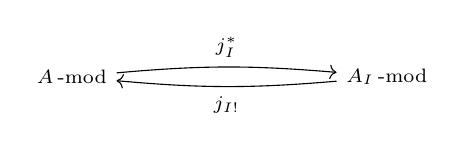
\begin{tikzpicture}
\node (v1) at (0,0) {\scriptsize ${{\PiQ}\module}$};
\node (v2) at (4,0) {\scriptsize ${{\PiQ_I}\module}$};

\draw [->,bend right=-5] (v1) to node[above] {$\scriptstyle{j_I^*}$} (v2);
\draw [->,bend left=5] (v2) to node[below] {$\scriptstyle{j_{I!}}$} (v1);
\end{tikzpicture}
\]
 defined by $j_I^*(-)\coloneqq \overline{e}_I \PiQ \otimes_{\PiQ} (-)$ and $j_{I!}(-)\coloneqq \PiQ \overline{e}_I\otimes_{\PiQ_I}(-)$. These are two of the six functors in a recollement of the module category ${\PiQ}\module$ \cite[Section 3]{craw2018multigraded}. In particular, $j_I^*$ is exact, $j_I^*j_{I!}$ is the identity functor, and for any $\PiQ_I$-module $N$, the $\PiQ$-module $j_{I!}(N)$ provides the maximal extension by $\PiQ/(\PiQ \overline{e}_I\PiQ)$-modules.

\begin{Lemma}\label{lem:j!semistable}
Let $N$ be an $\eta_I$-stable $\PiQ_I$-module of dimension vector $(1,n_I)$. Then $j_{I!}(N)$ is a~$\theta_I$-semistable $\PiQ$-module of finite dimension satisfying $\dim_i j_{I!}(N)=\dim_i N$ for $i \in \{\infty\} \cup I$.
\end{Lemma}
\begin{proof}The proofs of \cite[Lemma~4.4 and Lemma~4.5]{craw2019punctual} do not rely on the choice of dimension vector, so they apply equally well for the vector $(1,n_I)$.
\end{proof}

This gives the following partial converse to the Proposition~\ref{prop:key}.

 \begin{Corollary} Suppose that $\mathcal{M}_{A_I}(1,n_I)$ is non-empty. There exists $v\in \mathbb{N}^{r+1}$ satisfying $v_i=n_i$ for all $i \in I$ such that $\mathfrak{M}_{\theta_I}(1,v)$ is non-empty.
 \end{Corollary}
 \begin{proof}
 Let $N$ denote an $\eta_I$-stable $A_I$-module of dimension vector $(1,n_I)$. Lemma~\ref{lem:j!semistable} shows that $j_{I!}(N)$ is a $\theta_I$-semistable $A$-module of dimension vector $(1,v)$, where $v\in \mathbb{N}^{r+1}$ satisfies $v_i=n_i$ for all $i\in I$. In particular, $\mathfrak{M}_{\theta_I}(1,v)\neq \varnothing$.
 \end{proof}

 \begin{Lemma} \label{lem:existsemistable} Let $N$ be an $\eta_I$-stable $\PiQ_I$-module of dimension vector $(1,n_I)$ and let $(1,v) \in \mathcal{V}(n_I)$ be any vector such that $\mathfrak{M}_{\theta_I}(1,v)$ is non-empty. Choose
$\widetilde{v}$ as in Proposition~{\rm \ref{prop:surjvar}}. Then there exists a $\theta_I$-semistable $\PiQ$-module $M$ such that $j_I^*M \cong N$ with $\dim_{\infty} M =1$, $\dim_i M = n_i$ for all $i\in I$ and $\dim_k M \leq \widetilde{v}_k$ for all $k\in K\coloneqq\{0,1,\dots,r\}\setminus I$.
 \end{Lemma}

\begin{proof} Lemma~\ref{lem:j!semistable} shows that $j_{I!}(N)$ is $\theta_I$-semistable. If $\dim_i j_{I!}(N) \leq \widetilde{v}_i$ for $i\not\in \{\infty\}\cup I$, then
 $M\coloneqq j_{I!}(N)$ is the required $A$-module because $j_I^*j_{I!}$ is the identity. Otherwise, consider the $\theta_I$-polystable module $\bigoplus_{\lambda} M_\lambda$ that is $S$-equivalent to $j_{I!}(N)$. Let $M_{\lambda_\infty}$ denote the unique summand satisfying $\dim_\infty M_{\lambda_\infty} =1$. By Lemma~\ref{lem:j!semistable}, we have $\dim_i j_!(N) = n_i$, so $\dim_i M_{\lambda_\infty} \le n_i$.
 If $\dim_i M_{\lambda_\infty}<n_i$ for some $i\in I$, we would have $\theta_I(M_{\lambda_\infty})<0$, contradicting the
 $\theta_I$-stability of~$M_{\lambda_\infty}$. It follows that $\dim_i M_{\lambda_\infty} =n_i$ for all $i\in I$, and hence $\dim_i M_\lambda =0$ for all $\lambda\neq {\lambda_\infty}$ and all $i\in \{\infty\}\cup I$. For each index $\lambda$ and all $i\in \{\infty\}\cup I$, we have
\[
\dim_i j_I^*M_\lambda = \dim e_i \big(\overline{e}_I\PiQ\otimes_{\PiQ}(M_\lambda)\big) = \dim e_i \PiQ\otimes_{\PiQ} M_\lambda = \dim_i M_\lambda,
\]
 so $\dim_i j_I^*M_\lambda = 0$ for all
 $\lambda\neq {\lambda_\infty}$ and $i\in \{\infty\}\cup I$, and hence
 $j_I^*M_\lambda=0$ for $\lambda\neq {\lambda_\infty}$.

 We claim that $j_I^*M_{\lambda_\infty}$ is isomorphic to $N$. Indeed, the $\PiQ$-module $j_{I!}(N)$ is $\theta_I$-semistable by Lemma~\ref{lem:j!semistable}, and the $\theta_I$-stable $\PiQ$-modules $M_\lambda$ are
 the factors in the composition series of~$j_{I!}(N)$ in the category of $\theta_I$-semistable $\PiQ$-modules. It follows from exactness of $j_I^*$ that the $\PiQ_I$-modules~$j_I^*M_\lambda$ are the factors in the composition series of $j_I^*j_{I!}(N)\cong N$ in the category of $\eta_I$-semistable $\PiQ_I$-modules. But $j_I^*M_\lambda=0$ for $\lambda\neq {\lambda_\infty}$, so the only nonzero factor of the composition series is $j_I^*M_{\lambda_\infty}$. It follows that $j_I^*M_{\lambda_\infty}\cong N$, because the factor $j_I^*M_{\lambda_\infty}$ can only appear once in the composition series.

 We established above that
 $\dim_\infty M_{\lambda_\infty} =1$ and $\dim_i M_{\lambda_\infty} = n_i$ for all $i\in I$.
 Thus, to show that $M_{\lambda_\infty}$ is the required $A$-module, it remains to check that
 \begin{equation*}% \label{eqn:dimMlambdainfty}
 \dim_k M_{\lambda_\infty} \leq \widetilde{v}_k
 \end{equation*}
 for $k\in K=\{0,1,\dots,r\}\setminus I$.
 To simplify notation, write
 $(1,w)\coloneqq \dim M_{\lambda_\infty}$ for some $ w \in \SN^{r+1}$. We first establish the weaker inequality $ w \leq v$ (recall that $\widetilde{v} \leq v$ by Proposition~\ref{prop:surjvar}).
Combine the inequalities on the components of $v$ coming from the assumption $(1,v)\in \mathcal{V}(n_I)$, together with the inequalities on the components of $(1,w)$ obtained by applying Lemma~\ref{lem:Vnj} to the $\theta_I$-stable $\PiQ_I$-module $M_{\lambda_\infty}$, to obtain the inequality
 \begin{equation} \label{eqn:v-wk}
 2(v-w)_k \geq \sum_{\{e \in Q_1\mid \tail(e)=k\}} (v-w)_{\head(e)}
 \end{equation}
 for all $k \in K\coloneqq \{0,\dots,r\}\setminus I$.
 The vertex set $K$, together with all edges of the ADE Dynkin diagram joining two vertices from $K$, is
 a disjoint union of simply laced Dynkin diagrams. Let~$\Lambda$ be one of these subdiagrams, and let $C$ be its Cartan matrix. It follows from \eqref{eqn:v-wk} that $C(v-w)|_\Lambda\geq 0$. But the matrix $C^{-1}$ only has nonnegative entries (see, for example, \cite[equations~(1.157)--(1.158)]{Rosenfeld}), so $(v-w)|_\Lambda=C^{-1}C(v-w)|_\Lambda\ge 0$. Combining these inequalities for every such subdiagram $\Lambda$ with the equalities $ w_i=v_i$ for $i\in \{\infty\}\cup I$ gives $v\ge w$. This shows that $v_k-w_k\geq 0$ for all $k\in K$. Let $S_k\coloneqq\SC e_k$ denote the vertex simple $A$-module at vertex $k\in K$. The $\PiQ$-module
 \[
 \overline{M}\coloneqq M_{\lambda_\infty}\oplus \bigoplus_{k\in K}
 S_k^{\oplus (v_k-w_k)}
 \]
 is $\theta_I$-semistable of dimension vector $(1,v)$ by construction. As $M_{\lambda_\infty}$ is the unique summand of $\overline{M}$ with
dimension 1 at the vertex $\infty$, we have $w \leq \widetilde{v}$ by Lemma~\ref{lem:vwtildev}.
 \end{proof}

\begin{Theorem}\label{thm:mthetamorph1}
Let $v=(v_j)_{0 \leq j \leq r} \in \mathbb{N}^{r+1}$ be any vector satisfying $v_i=n_i$ for all $i \in I$. Suppose that $\mathfrak{M}_{\theta_I}(1,v)$ is non-empty. For the vector $(1,\vprime)\in \mathcal{V}(n_I)$ from Corollary~{\rm \ref{cor:non-empty}}, choose a vector~$\widetilde{\vprime}$ as in Proposition~{\rm \ref{prop:surjvar}}. Then
there is a commutative diagram
\begin{equation}\label{eqn:keyrevisited}
\begin{tikzcd}
 & \mathfrak{M}_{\widetilde{\theta}}\big(1, \widetilde{\vprime}\big) \arrow[dl, "\pi_I", swap ] \arrow[dr, "\tau_I" ]& \\
 \mathfrak{M}_{\theta_I}(1, \vprime) \arrow[rr, "\iota_I" ] & & \mathcal{M}_{\PiQ_I} (1,n_I)
\end{tikzcd}
\end{equation}
 of schemes over $\C$, where $\iota_I$ is an isomorphism of the underlying reduced schemes. Thus, $\mathcal{M}_{\PiQ_I}(1,n_I)$ is non-empty, irreducible, and its
underlying reduced scheme is normal and has symplectic singularities.
\end{Theorem}
 \begin{proof}
Note first that $\mathfrak{M}_{\theta_I}(1,\vprime)$ is non-empty by Corollary~\ref{cor:non-empty}, so we may indeed apply Proposition~\ref{prop:surjvar} to obtain the vector $\widetilde{\vprime}$. The diagram
 from Proposition~\ref{prop:key} now takes the form as shown in \eqref{eqn:keyrevisited}. To prove that $\iota_I$ is an isomorphism of the underlying reduced schemes, it suffices to show that $\iota_I$ is surjective on closed points. The diagram commutes, $\pi_I$ is surjective and $\iota_I$ is a~closed immersion, so it suffices to show that $\tau_I$ is surjective on closed points. Consider a closed point $[N]\in \mathcal{M}_{\PiQ_I}(1,n_I)$, where $N$ is an $\eta_I$-stable $\PiQ_I$-module of dimension vector $(1,n_I)$. Let $M$ be the $\theta_I$-semistable $\PiQ$-module from Lemma~\ref{lem:existsemistable}. Since
 \[
 m_k\coloneqq {\vprime_k}-\dim_k M \geq {\widetilde{\vprime_k}} - \dim_k M \geq 0
 \]
 for all $k\in K=\{0,1,\dots,r\}\setminus I$ by Proposition~\ref{prop:surjvar} and Lemma~\ref{lem:existsemistable}, we may once again define
 \[
 \overline{M}\coloneqq M\oplus \bigoplus_{k\in K} S_k^{\oplus m_k},
 \]
 where
 $S_k$ is the vertex simple $A$-module at vertex $k\in K=\{0,\dots,r\}\cup I$. The $\PiQ$-module $ \overline{M}$ is $\theta_I$-semistable of dimension vector $(1,\vprime)$ by construction, and it satisfies $j_I^*(\overline{M}) = j_I^*(M) = N$. Write $[\overline{M}]\in \mathfrak{M}_{\theta_I}(1,\vprime)$ for the corresponding closed point, and let $\widetilde{M}$ be any $\widetilde{\theta}$-stable $A$-module of dimension vector $\big(1, \widetilde{\vprime}\big)$ such that the closed point $[\widetilde{M}]\in \mathfrak{M}_{\widetilde{\theta}}\big(1, \widetilde{\vprime}\big)$ satisfies $\pi_I([\widetilde{M}])=[\overline{M}]\in \mathfrak{M}_{\theta_I}(1,\vprime)$. Then $j_I^*(\widetilde{M})=j_I^*(\overline{M})=N$, hence $\tau_I([\widetilde{M}])= [N]$.
 The final statement of the proposition follows from Lemma~\ref{lem:quiver} and Proposition~\ref{prop:key}.
 \end{proof}
\begin{thebibliography}{99}
\bibitem[3]{bellamy2020birational}
Bellamy G., Craw A., Birational geometry of symplectic quotient singularities,
 \href{https://doi.org/10.1007/s00222-020-00972-9}{\textit{Invent. Math.}} \textbf{222} (2020), 399--468, \href{https://arxiv.org/abs/1811.09979}{arXiv:1811.09979}.

\bibitem[4]{bellamy2016symplectic}
Bellamy G., Schedler T., Symplectic resolutions of quiver varieties,
 \href{https://doi.org/10.1007/s00029-021-00647-0}{\textit{Selecta Math.~(N.S.)}} \textbf{27} (2021), 36, 50~pages,
 \href{https://arxiv.org/abs/1602.00164}{arXiv:1602.00164}.

\bibitem[7]{craw2019punctual}
Craw A., Gammelgaard S., Gyenge \'A., Szendr\H{o}i B., Punctual {H}ilbert schemes
 for {K}leinian singularities as quiver varieties, \href{https://doi.org/10.14231/AG-2021-021}{\textit{Algebr. Geom.}}
 \textbf{8} (2021), 680--704, \href{https://arxiv.org/abs/1910.13420}{arXiv:1910.13420}.

\bibitem[8]{craw2018multigraded}
Craw A., Ito Y., Karmazyn J., Multigraded linear series and recollement,
 \href{https://doi.org/10.1007/s00209-017-1965-1}{\textit{Math.~Z.}} \textbf{289} (2018), 535--565, \href{https://arxiv.org/abs/1701.01679}{arXiv:1701.01679}.

\bibitem[10]{dehority2020affinizations}
DeHority S., Affinizations of {L}orentzian {K}ac--{M}oody algebras and
 {H}ilbert schemes of points on {$K3$} surfaces, \href{https://arxiv.org/abs/2007.04953}{arXiv:2007.04953}.

\bibitem[11]{goodman2009symmetry}
Goodman R., Wallach N.R., Symmetry, representations, and invariants,
 \textit{Graduate Texts in Mathematics}, Vol.~255, \href{https://doi.org/10.1007/978-0-387-79852-3}{Springer}, Dordrecht, 2009.

\bibitem[13]{gyenge2018euler}
Gyenge \'A., N\'emethi A., Szendr\H{o}i B., Euler characteristics of {H}ilbert
 schemes of points on simple surface singularities, \href{https://doi.org/10.1007/s40879-018-0222-4}{\textit{Eur.~J. Math.}}
 \textbf{4} (2018), 439--524, \href{https://arxiv.org/abs/1512.06848}{arXiv:1512.06848}.

\bibitem[14]{hartshorne1977algebraic}
Hartshorne R., Algebraic geometry, \textit{Graduate Texts in Mathematics},
 Vol.~52, \href{https://doi.org/10.1007/978-1-4757-3849-0}{Springer-Verlag}, New York~-- Heidelberg, 1977.

\bibitem[15]{king1994moduli}
King A.D., Moduli of representations of finite-dimensional algebras,
 \href{https://doi.org/10.1093/qmath/45.4.515}{\textit{Quart.~J. Math. Oxford}} \textbf{45} (1994), 515--530.

\bibitem[16]{kuznetsov2007quiver}
Kuznetsov A., Quiver varieties and {H}ilbert schemes, \href{https://doi.org/10.17323/1609-4514-2007-7-4-673-697}{\textit{Mosc. Math.~J.}}
 \textbf{7} (2007), 673--697, \href{https://arxiv.org/abs/math.AG/0111092}{arXiv:math.AG/0111092}.

\bibitem[18]{McKay80}
McKay J., Graphs, singularities, and finite groups, in The {S}anta {C}ruz
 {C}onference on {F}inite {G}roups ({U}niv. {C}alifornia, {S}anta {C}ruz,
 {C}alif., 1979), \textit{Proc. Sympos. Pure Math.}, Vol.~37, Amer. Math.
 Soc., Providence, R.I., 1980, 183--186.

\bibitem[19]{nakajima1994instantons}
Nakajima H., Instantons on {ALE} spaces, quiver varieties, and {K}ac--{M}oody
 algebras, \href{https://doi.org/10.1215/S0012-7094-94-07613-8}{\textit{Duke Math.~J.}} \textbf{76} (1994), 365--416.

\bibitem[20]{Nakajima98}
Nakajima H., Quiver varieties and {K}ac--{M}oody algebras, \href{https://doi.org/10.1215/S0012-7094-98-09120-7}{\textit{Duke
 Math.~J.}} \textbf{91} (1998), 515--560.

\bibitem[21]{nakajima2002geometric}
Nakajima H., Geometric construction of representations of affine algebras, in
 Proceedings of the {I}nternational {C}ongress of {M}athematicians, {V}ol.~{I}
 ({B}eijing, 2002), Higher Ed. Press, Beijing, 2002, 423--438.

\bibitem[22]{nakajima2009quiver}
Nakajima H., Quiver varieties and branching, \href{https://doi.org/10.3842/SIGMA.2009.003}{\textit{SIGMA}} \textbf{5} (2009),
 003, 37~pages, \href{https://arxiv.org/abs/0809.2605}{arXiv:0809.2605}.

\bibitem[24]{Rosenfeld}
Rosenfeld B., Geometry of {L}ie groups, \textit{Mathematics and its
 Applications}, Vol.~393, \href{https://doi.org/10.1007/978-1-4757-5325-7}{Kluwer Academic Publishers Group}, Dordrecht, 1997.

\bibitem[25]{savage2011quiver}
Savage A., Tingley P., Quiver {G}rassmannians, quiver varieties and the
 preprojective algebra, \href{https://doi.org/10.2140/pjm.2011.251.393}{\textit{Pacific~J. Math.}} \textbf{251} (2011),
 393--429, \href{https://arxiv.org/abs/0909.3746}{arXiv:0909.3746}.

\end{thebibliography}
\end{document}
